\chapter{Olahraga dan Kebutuhan Energi Tubuh}\label{ch:g10:exercise-and-energy}

Seorang pesepeda di atas sepeda laboratorium mengayuh melawan rem yang
mengukur dayanya: \qty{100}{W}, lalu \qty{150}{W}, lalu \qty{200}{W}.
Sebuah masker menutupi wajahnya dan mengirim tiap embusan napasnya ke
penganalisis. Angka di layarnya memanjat seiring remnya: makin banyak
usaha mekanis yang diberikannya, makin banyak oksigen yang dipakainya
dan makin banyak karbon dioksida yang diembuskannya. Ototnya sedang
menjalankan respirasi \cref{ch:g10:cell-metabolism} dengan
sepenuh-penuhnya, dan penganalisisnya sedang membaca neracanya. Bab ini
mengikuti energi olahraga dari makanan yang memasoknya sampai oksigen
yang melepaskannya.

\section{Energi masuk, usaha keluar}

\begin{definition}[Pengeluaran energi]\label{def:g10:exercise-and-energy:expenditure}
Yang disebut \emph{pengeluaran energi}\index{pengeluaran energi} tubuh,
dalam joule, adalah seluruh energi yang dilepaskan \omterm{def:g10:cells-common-unit:cell}{selnya} dari molekul
organik selama waktu tertentu. Dibagi waktunya, ia menjadi
\emph{daya \omterm{def:g10:cell-metabolism:metabolism}{metabolisme}}, dalam watt. Dalam keadaan istirahat, orang
dewasa mengeluarkan sekitar \qty{80}{W} --- sekitar \qty{7000}{kJ}
sehari --- untuk menjaga jantungnya berdenyut, otaknya bekerja, suhunya
pada \qty{37}{\celsius} dan \omterm{def:g10:cells-common-unit:cell}{selnya} tetap hidup; inilah
\emph{\omterm{def:g10:cell-metabolism:metabolism}{metabolisme} basal}. Setiap kegiatan menambahinya.
\end{definition}

\begin{proposition}[Ke mana energinya pergi]\label{prop:g10:exercise-and-energy:efficiency}
Otot yang bekerja mengubah hanya sekitar seperempat energi yang
dilepaskannya menjadi usaha mekanis; tiga perempat sisanya keluar
sebagai kalor. Karena itu memberikan daya mekanis $P$ menuntut tubuh
mengeluarkan daya \omterm{def:g10:cell-metabolism:metabolism}{metabolisme} sekitar $4P$ di atas keadaan istirahat:
pesepeda pada \qty{100}{W} di pedalnya mengeluarkan sekitar
\qty{400}{W} dalam ototnya, dan tubuhnya harus membuang \qty{300}{W}
kalor --- sebagian besar lewat berkeringat.
\end{proposition}
\admitted

\begin{example}[Anggaran harian]\label{ex:g10:exercise-and-energy:budgets}
Seorang murid yang duduk di kelas, berjalan ke sekolah dan tidur
mengeluarkan sekitar \qty{9000}{kJ} sehari; satu jam sepak bola
menambahkan sekitar \qty{2500}{kJ}; sehari di pegunungan dengan ransel,
\qty{15000}{kJ} seluruhnya. Pesepeda pada etape pegunungan sebuah lomba
mengeluarkan \qty{25000}{kJ}, dan tidak dapat makan cukup banyak
sepanjang hari untuk menutupinya. Energinya berasal dari makanan
(\cref{ch:g10:chemistry-of-life}): \qty{17}{kJ} tiap gram \omterm{def:g10:chemistry-of-life:families}{karbohidrat}
atau \omterm{def:g10:chemistry-of-life:families}{protein}, \qty{38}{kJ} tiap gram \omterm{def:g10:chemistry-of-life:families}{lipid}.
\end{example}

\section{Pemakaian oksigen mengukur pengeluaran energi}

\begin{proposition}[Kesetaraan oksigennya]\label{prop:g10:exercise-and-energy:oxygen}
Karena energi olahraga dilepaskan lewat \omterm{prop:g10:cell-metabolism:respiration}{respirasi seluler}, yang memakai
oksigen, konsumsi oksigen tubuh mengukur \omterm{def:g10:exercise-and-energy:expenditure}{pengeluaran energinya}: tiap
liter oksigen yang terpakai sepadan dengan sekitar \qty{20}{kJ} yang
dilepaskan, apa pun campuran glukosa dan \omterm{def:g10:chemistry-of-life:families}{lipid} yang dibakar. Dalam
keadaan istirahat seseorang memakai sekitar \qty{0.25}{L} oksigen tiap
menit; selama olahraga pemakaiannya naik sebanding dengan daya yang
diberikan, sampai ke batas atas pribadinya.
\end{proposition}
\begin{proof}[Bukti percobaan]
Persamaan respirasi pada \cref{ch:g10:cell-metabolism} memberi
\qty{2870}{kJ} untuk \qty{6}{mol} oksigen, yaitu \qty{478}{kJ} tiap mol,
dan satu mol gas menempati sekitar \qty{24}{L}: \qty{20}{kJ} tiap liter.
Untuk \omterm{def:g10:chemistry-of-life:families}{lipid} angkanya \qty{19.6}{kJ/L}, untuk \omterm{def:g10:chemistry-of-life:families}{karbohidrat}
\qty{21.1}{kJ/L}, sehingga campurannya nyaris tidak berpengaruh.
Pengukuran dalam bilik tertutup, tempat kalor yang dilepaskan seorang
subjek dikumpulkan langsung, sesuai dengan angka oksigennya sampai
beberapa persen.
\end{proof}

\begin{omfigure}
\begin{tikzpicture}
\begin{axis}[
  width=0.86\linewidth, height=5.8cm,
  axis x line=bottom, axis y line=left,
  xmin=0, xmax=320, ymin=0, ymax=4.2,
  xlabel={daya mekanis (W)}, ylabel={$\mathrm{O_2}$ terpakai (L/min)},
  xlabel style={font=\small, at={(axis description cs:0.5,-0.12)}, anchor=north},
  ylabel style={font=\small},
  tick label style={font=\small},
  xtick={0,50,100,150,200,250,300}, ytick={0,1,2,3,4},
  clip=false,
]
\addplot[thick, omThm, mark=*, mark size=1.6pt] coordinates
  {(0,0.3) (50,0.9) (100,1.5) (150,2.1) (200,2.7) (250,3.2) (300,3.3)};
\draw[dashed, gray] (axis cs:0,3.3) -- (axis cs:320,3.3);
\node[font=\small, anchor=south east] at (axis cs:318,3.32) {$\dot V\!\mathrm{O_2}$maks};
\node[font=\small, anchor=south west, align=left] at (axis cs:40,3.42) {kemiringan: \qty{12}{mL} $\mathrm{O_2}$ tiap menit\\ untuk tiap watt};
\end{axis}
\end{tikzpicture}

{\small Konsumsi oksigen seorang subjek yang mengayuh dengan daya yang
meningkat. Kenaikannya linear --- sekitar \qty{12}{mL} oksigen tiap
menit tiap watt --- sampai konsumsinya mencapai batas atasnya, yaitu
$\dot V\!\mathrm{O_2}$maks subjek itu; di luar batas itu daya
tambahannya dipasok tanpa oksigen dan tidak dapat dipertahankan.}
\end{omfigure}

\begin{definition}[Konsumsi oksigen maksimal]\label{def:g10:exercise-and-energy:vo2max}
Yang disebut \emph{konsumsi oksigen maksimal}\index{konsumsi oksigen
maksimal}, yang ditulis $\dot V\!\mathrm{O_2}$maks, adalah laju
tertinggi yang dengannya tubuh seseorang dapat menyerap dan memakai
oksigen, dalam liter tiap menit --- atau, untuk membandingkan orang
yang berbeda ukurannya, dalam mililiter tiap menit tiap kilogram massa
tubuh. Ia menetapkan daya tertinggi yang dapat dipertahankan oleh
respirasi saja. Nilai yang lazim: \qty{35}{mL/min} tiap kilogram pada
orang dewasa yang kurang gerak, \num{50} pada murid yang terlatih,
\num{80} atau lebih pada juara olahraga ketahanan.
\end{definition}

\begin{example}[Membaca lengkungnya]\label{ex:g10:exercise-and-energy:reading}
Pada gambarnya, mengayuh \qty{100}{W} menuntut \qty{1.5}{L/min}
oksigen: $1.5 \times 20 = \qty{30}{kJ}$ tiap menit, yaitu \qty{500}{W}
daya \omterm{def:g10:cell-metabolism:metabolism}{metabolisme} --- yaitu \qty{100}{W} usaha ditambah \qty{400}{W}
kalor dan kebutuhan istirahat, sejalan dengan
\cref{prop:g10:exercise-and-energy:efficiency}. Batas atas
\qty{3.3}{L/min} bagi subjek \qty{66}{kg} sama dengan \qty{50}{mL/min}
tiap kilogram.
\end{example}

\begin{omfigure}
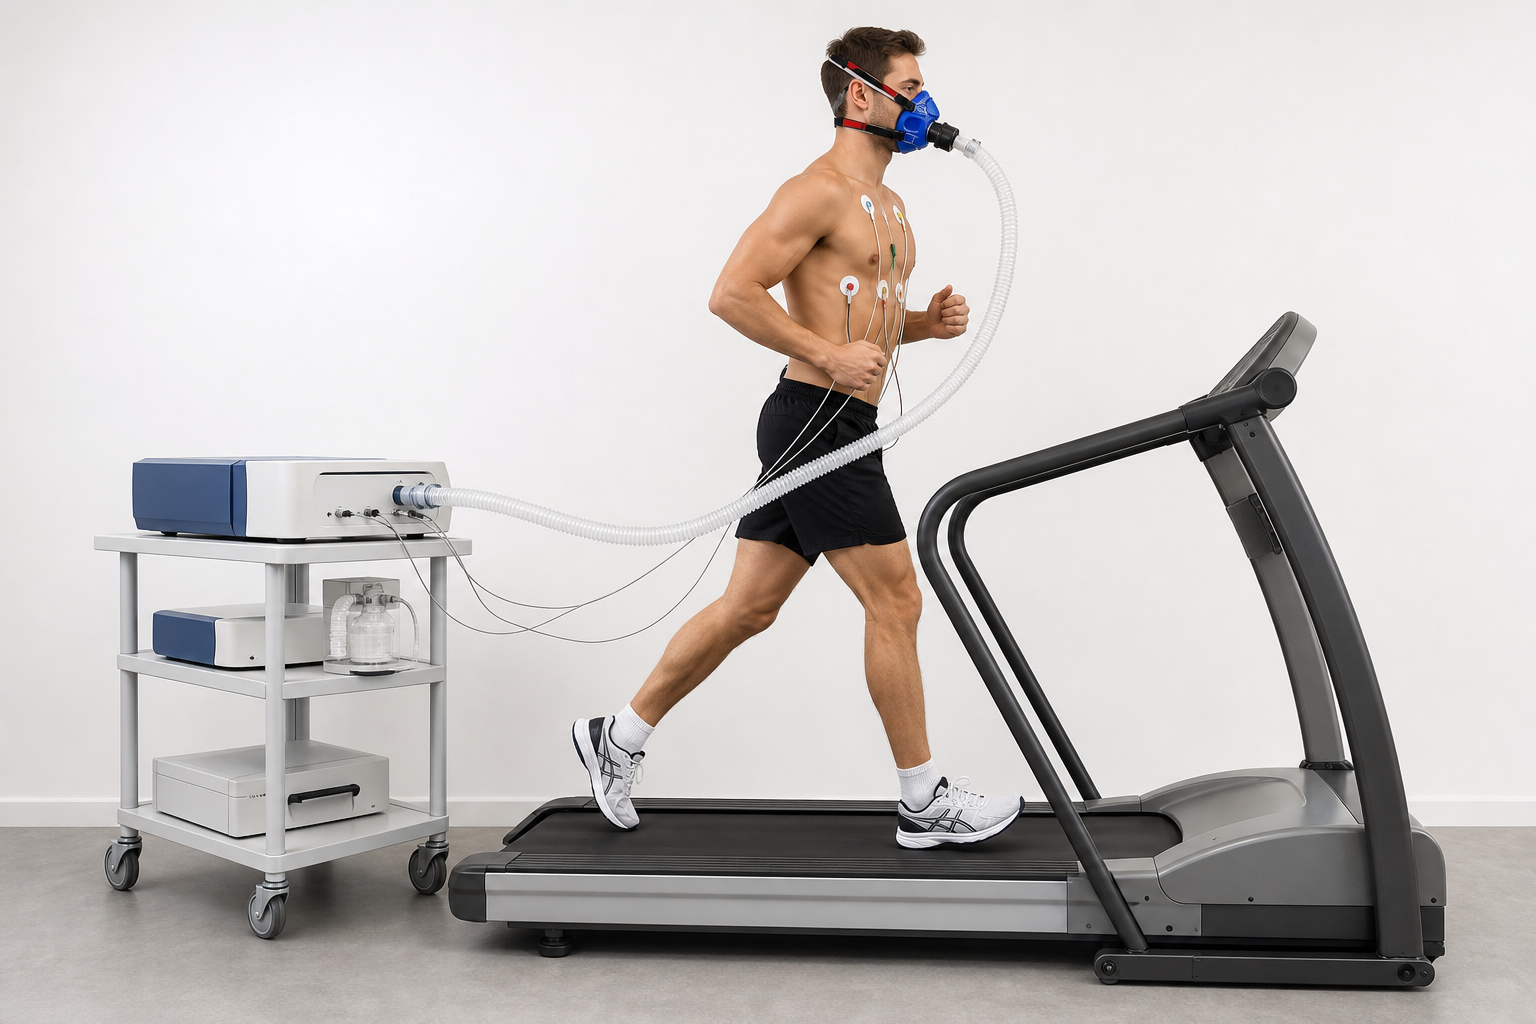
\includegraphics[width=0.62\linewidth]{images/book2/ai/g10-exercise-treadmill-mask.png}

{\small Mengukur konsumsi oksigen selama olahraga: tiap embusan napas
melewati masker menuju penganalisis gas yang merekam oksigen yang
terserap dan karbon dioksida yang dilepaskan, menit demi menit,
sementara ban berjalannya menetapkan dayanya.}
\end{omfigure}

\section{Bahan bakar otot}

\begin{proposition}[Tiga sumber ATP]\label{prop:g10:exercise-and-energy:fuels}
Kerutan otot dibayar dengan ATP, dan \omterm{def:g10:cells-common-unit:cell}{selnya} hanya menyimpan persediaan
untuk beberapa sekon. ATP-nya diperbarui lewat tiga jalur, yang
masing-masing punya kecepatan dan kapasitasnya sendiri:
\begin{itemize}
  \item simpanan kecil sebuah senyawa fosfat dalam ototnya, yang
        membentuk ulang ATP seketika tetapi bertahan sekitar sepuluh
        sekon --- untuk lari cepat;
  \item \omterm{def:g10:cell-metabolism:fermentation}{fermentasi} laktat glukosa dalam \omterm{def:g10:cells-common-unit:cell}{sitoplasma}, yang cepat tetapi
        boros, yang menopang usaha habis-habisan selama satu sampai dua
        menit dan menghasilkan asam laktat;
  \item \omterm{prop:g10:cell-metabolism:respiration}{respirasi seluler} dalam \omterm{def:g10:cells-common-unit:organelle}{mitokondria}, yang lebih lambat mencapai
        laju penuh tetapi hampir tak terbatas lamanya, yang membakar
        glukosa dari darah, \omterm{def:g10:exercise-and-energy:glycogen}{glikogen} dari otot, dan asam lemak dari
        lemak tubuh.
\end{itemize}
Bagian masing-masing bergantung pada kegiatan dan lamanya olahraganya.
\end{proposition}
\admitted

\begin{omfigure}
\begin{tikzpicture}
\begin{axis}[
  ybar stacked, bar width=18pt,
  width=0.86\linewidth, height=5.6cm,
  axis x line=bottom, axis y line=left,
  ymin=0, ymax=100, ylabel={bagian energinya (\%)}, ylabel style={font=\small},
  symbolic x coords={10 s, 1 min, 4 min, 30 min, 2 h},
  xtick=data, tick label style={font=\small},
  xlabel={lama sebuah usaha habis-habisan},
  xlabel style={font=\small, at={(axis description cs:0.5,-0.12)}, anchor=north},
  enlarge x limits=0.15,
  legend style={at={(0.5,-0.3)}, anchor=north, legend columns=3,
                font=\small, draw=none},
]
\addplot[fill=omThm!50, draw=omThm] coordinates {(10 s,85) (1 min,25) (4 min,8) (30 min,2) (2 h,1)};
\addplot[fill=omProp!50, draw=omProp] coordinates {(10 s,12) (1 min,50) (4 min,32) (30 min,8) (2 h,2)};
\addplot[fill=omDef!50, draw=omDef] coordinates {(10 s,3) (1 min,25) (4 min,60) (30 min,90) (2 h,97)};
\legend{simpanan fosfat, fermentasi laktat, respirasi}
\end{axis}
\end{tikzpicture}

{\small Bagian hampiran ketiga sumber ATP dalam usaha habis-habisan
yang lamanya tertentu. Lari cepat 100 meter berjalan dengan simpanan
fosfat; lomba 400 meter sebagian besar dengan \omterm{def:g10:cell-metabolism:fermentation}{fermentasi}; apa pun yang
melampaui beberapa menit dengan respirasi.}
\end{omfigure}

\begin{definition}[Glikogen]\label{def:g10:exercise-and-energy:glycogen}
Yang disebut \emph{glikogen}\index{glikogen} adalah bentuk hewani
\omterm{def:g10:chemistry-of-life:families}{karbohidrat} yang tersimpan: rantai satuan glukosa yang bercabang, yang
tersimpan sebagai butiran dalam \omterm{def:g10:cells-common-unit:cell}{sel} otot (sekitar \qty{400}{g} pada
orang dewasa) dan dalam hati (sekitar \qty{100}{g}). Glikogen otot
menjadi bahan bakar otot yang menyimpannya; glikogen hati dibongkar
menjadi glukosa yang dilepaskan ke dalam darah, yang menjaga glukosa
darahnya mendekati \qty{1}{g/L} bagi otak dan jaringan lainnya. Lemak,
yang tersimpan dalam \omterm{def:g10:cells-common-unit:cell}{sel} lemak, adalah cadangan yang jauh lebih besar
(\cref{ch:g10:chemistry-of-life}), tetapi ia hanya dapat dibakar dengan
lambat dan hanya dengan oksigen.
\end{definition}

\begin{example}[Tembok maraton]\label{ex:g10:exercise-and-energy:wall}
Berlari menuntut sekitar \qty{4}{kJ} tiap kilogram massa tubuh tiap
kilometer; pelari \qty{70}{kg} mengeluarkan \qty{280}{kJ/km}, dan satu
maraton menuntut \qty{11800}{kJ}. Simpanan \omterm{def:g10:exercise-and-energy:glycogen}{glikogennya} memuat sekitar
\qty{8500}{kJ}. Jika pelarinya membakar \omterm{def:g10:exercise-and-energy:glycogen}{glikogen} terlalu cepat,
simpanannya habis sekitar kilometer ketiga puluh; ototnya lalu harus
bersandar pada lemak, yang memasok energi dengan laju nyaris separuhnya
saja, dan kecepatannya runtuh --- ``menabrak tembok''. Pelari yang
terlatih membakar bagian lemak yang lebih besar sejak awal, dan makan
\omterm{def:g10:chemistry-of-life:families}{karbohidrat} selama lombanya.
\end{example}

\begin{omfigure}
\begin{tikzpicture}[>=Stealth, font=\small,
  b/.style={draw, rounded corners, align=center, minimum height=0.9cm, text width=2.5cm}]
  \node[b, fill=omDef!12] (food) at (0,2.2) {makanan:\\ karbohidrat, lipid};
  \node[b, fill=omDef!12] (gly) at (0,0.6) {glikogen (otot,\\ hati), glukosa darah};
  \node[b, fill=omDef!12] (fat) at (0,-1.0) {asam lemak\\ dari lemak tubuh};
  \node[b, fill=omThm!12, minimum height=2.6cm] (mit) at (4.3,-0.2) {mitokondria:\\ respirasi};
  \node[b, fill=omProp!15] (o2) at (4.3,2.2) {oksigen, dari\\ paru-paru dan darah};
  \node[b, fill=omMeth!15] (atp) at (9.2,-0.2) {ATP};
  \node[b, fill=white] (work) at (12.5,0.8) {usaha otot\\ (sekitar 25\%)};
  \node[b, fill=white] (heat) at (12.5,-1.2) {kalor\\ (sekitar 75\%)};
  \draw[->] (food) -- (gly);
  \draw[->] (food.west) to[bend right=40] (fat.west);
  \draw[->] (gly) -- (mit);
  \draw[->] (fat) -- (mit);
  \draw[->] (o2) -- (mit);
  \draw[->] (mit) -- node[above, font=\scriptsize] {$\mathrm{CO_2}$ keluar} (atp);
  \draw[->] (atp) -- (work);
  \draw[->] (atp) -- (heat);
\end{tikzpicture}

{\small Rantai energi olahraga yang berkelanjutan: bahan bakar dari
makanan dan simpanan tubuh, oksigen dari pernapasan, ATP yang dibuat
dalam \omterm{def:g10:cells-common-unit:organelle}{mitokondria} dan dibelanjakan untuk berkerut --- tiga perempatnya
keluar sebagai kalor.}
\end{omfigure}

\section{Mengukur dan menalar}

\begin{method}[Sebuah hitungan energi untuk olahraga]\label{met:g10:exercise-and-energy:calc}
\begin{enumerate}
  \item Dari oksigennya: energi (\unit{kJ}) $=$ oksigen yang terpakai
        (\unit{L}) $\times 20$. Kurangi konsumsi istirahatnya jika
        pertanyaannya meminta biaya olahraganya saja.
  \item Dari daya mekanisnya: daya \omterm{def:g10:cell-metabolism:metabolism}{metabolisme} $\approx 4 P$; energi
        $=$ daya $\times$ waktu (\qty{1}{W} selama \qty{1}{s} sama
        dengan \qty{1}{J}; \qty{1}{kWh} $= \qty{3600}{kJ}$).
  \item Dari bahan bakarnya: massa yang terbakar $=$ energi $/$ nilai
        energinya (\qty{17}{kJ/g} \omterm{def:g10:chemistry-of-life:families}{karbohidrat}, \qty{38}{kJ/g} \omterm{def:g10:chemistry-of-life:families}{lipid});
        \omterm{def:g10:exercise-and-energy:glycogen}{glikogen} tersimpan bersama air tiga kali massanya.
  \item Periksa orde besarnya: sehari penuh sekitar \qty{10000}{kJ};
        satu jam yang berat, \qtyrange{2000}{3000}{kJ}; satu maraton,
        \qty{12000}{kJ}.
\end{enumerate}
\end{method}

\begin{example}[Satu jam bersepeda]\label{ex:g10:exercise-and-energy:hour}
Satu jam pada \qty{150}{W} di pedalnya: daya \omterm{def:g10:cell-metabolism:metabolism}{metabolismenya} sekitar
\qty{600}{W}, energinya $600 \times 3600 = \qty{2.16e6}{J} \approx
\qty{2200}{kJ}$; oksigennya $2200/20 = \qty{110}{L}$, yaitu \qty{1.8}{L/min}
--- sesuai dengan lengkungnya. Jika separuhnya berasal dari
\omterm{def:g10:chemistry-of-life:families}{karbohidrat}: $1100/17 \approx \qty{65}{g}$ glukosa atau \omterm{def:g10:exercise-and-energy:glycogen}{glikogen}, dan
$1100/38 \approx \qty{29}{g}$ lemak.
\end{example}

\begin{remark}[Mengapa oksigennya harus tiba]\label{rem:g10:exercise-and-energy:delivery}
Segala yang di atas mengandaikan bahwa oksigen mencapai \omterm{def:g10:cells-common-unit:organelle}{mitokondria}
secepat \omterm{def:g10:cells-common-unit:organelle}{mitokondria} dapat memakainya. Itulah tugas paru-paru, jantung
dan darah, yang tanggapannya terhadap olahraga --- napas yang lebih
cepat, denyut jantung yang lebih cepat dan lebih kuat, darah yang
dialihkan ke otot --- menjadi pokok \cref{ch:g10:heart-lungs-effort}.
$\dot V\!\mathrm{O_2}$maks sebagian besar adalah batas pengantarannya,
bukan batas selera ototnya.
\end{remark}

\section{Latihan}

\begin{exercise}[$\star$]\label{exo:g10:exercise-and-energy:1}
Rumuskan \omterm{def:g10:cell-metabolism:metabolism}{metabolisme} basal dan berikan orde besarnya dalam watt dan
dalam kilojoule tiap hari.
\end{exercise}

\begin{exercise}[$\star$]\label{exo:g10:exercise-and-energy:2}
Seorang subjek memakai \qty{2.0}{L} oksigen tiap menit. Berapa
\omterm{def:g10:exercise-and-energy:expenditure}{pengeluaran energinya} dalam kilojoule tiap menit, dan dalam watt?
\end{exercise}

\begin{exercise}[$\star$]\label{exo:g10:exercise-and-energy:3}
Sebutkan ketiga jalur yang dengannya otot memperbarui ATP-nya dan
berikan lama lazim yang dapat ditopang masing-masing sendirian.
\end{exercise}

\begin{exercise}[$\star$]\label{exo:g10:exercise-and-energy:4}
Apa itu $\dot V\!\mathrm{O_2}$maks? Setarakan \qty{3.5}{L/min} bagi
subjek \qty{70}{kg} menjadi mililiter tiap menit tiap kilogram.
\end{exercise}

\begin{exercise}[$\star$]\label{exo:g10:exercise-and-energy:5}
Di mana \omterm{def:g10:exercise-and-energy:glycogen}{glikogen} disimpan, dalam jumlah berapa, dan untuk apa tiap simpanannya?
\end{exercise}

\begin{exercise}[$\star\star$]\label{exo:g10:exercise-and-energy:6}
Dari gambar oksigen terhadap daya, bacalah konsumsi oksigennya pada
\qty{200}{W} dan hitung daya \omterm{def:g10:cell-metabolism:metabolism}{metabolismenya}. Turunkan kalor yang
dihasilkan tiap sekon.
\end{exercise}

\begin{exercise}[$\star\star$]\label{exo:g10:exercise-and-energy:7}
Seorang pendaki \qty{60}{kg} menanjak \qty{800}{m} dalam dua jam.
Hitung usaha mekanis melawan gravitasi ($g = \qty{9.8}{N/kg}$), energi
yang dikeluarkan ototnya jika efisiensinya 25\%, dan daya \omterm{def:g10:cell-metabolism:metabolism}{metabolisme}
rata-rata di atas keadaan istirahat.
\end{exercise}

\begin{exercise}[$\star\star$]\label{exo:g10:exercise-and-energy:8}
Dengan gambar batang bertumpuknya, jelaskan mengapa pelari 400 meter
terengah-engah dan nyeri di garis akhir sedangkan pelari cepat 100
meter nyaris tidak terengah.
\end{exercise}

\begin{exercise}[$\star\star$]\label{exo:g10:exercise-and-energy:9}
Seorang atlet mengeluarkan \qty{3000}{kJ} dalam satu sesi latihan, 60\%
darinya dari \omterm{def:g10:chemistry-of-life:families}{karbohidrat}. Berapa massa \omterm{def:g10:exercise-and-energy:glycogen}{glikogen} yang telah dipakainya,
dan berapa massa air yang dilepaskan bersamanya?
\end{exercise}

\begin{exercise}[$\star\star$]\label{exo:g10:exercise-and-energy:10}
Sebatang cokelat \qty{50}{g} menyediakan \qty{1100}{kJ}. Berapa lama ia
akan menenagai pesepeda yang mengayuh pada \qty{150}{W}?
\end{exercise}

\begin{exercise}[$\star\star$]\label{exo:g10:exercise-and-energy:11}
Mengapa suhu tubuh seseorang naik selama olahraga, dan dengan mekanisme
apa suhunya dicegah naik lebih jauh?
\end{exercise}

\begin{exercise}[$\star\star\star$]\label{exo:g10:exercise-and-energy:12}
Dua subjek bermassa \qty{60}{kg} dan \qty{90}{kg} sama-sama punya
$\dot V\!\mathrm{O_2}$maks \qty{3.6}{L/min}. Siapa yang dapat berlari
menanjak lebih cepat, dan siapa yang dapat mengayuh lebih kuat di jalan
datar pada sepeda laboratorium? Jelaskan.
\end{exercise}

\begin{exercise}[$\star\star\star$]\label{exo:g10:exercise-and-energy:13}
Konsumsi oksigen seorang pelari selama lomba adalah \qty{3.0}{L/min}
pada kecepatan yang, menurut lengkungnya, akan menuntut
\qty{3.4}{L/min}. Dari mana bedanya berasal, dan apa yang akan
dirasakan pelarinya setelah beberapa menit?
\end{exercise}

\begin{exercise}[$\star\star\star$]\label{exo:g10:exercise-and-energy:14}
Jelaskan mengapa seseorang tidak dapat mengurangi lemak lewat olahraga
pada kegiatan maksimal dalam letupan singkat seefektif lewat olahraga
sedang dalam waktu lama, dengan memakai ketiga jalur ATP-nya.
\end{exercise}

\begin{exercise}[$\star\star\star$]\label{exo:g10:exercise-and-energy:15}
Seorang pesepeda pada etape pegunungan mengeluarkan \qty{25000}{kJ}
dalam sehari. \omterm{def:g10:exercise-and-energy:glycogen}{Glikogennya} memuat \qty{8500}{kJ} dan ia makan
\qty{6000}{kJ} selama etapenya. Perkirakan massa lemak tubuh yang
dibakarnya, dan jelaskan mengapa pembalapnya makan terus-menerus selama
etape semacam itu.
\end{exercise}

\section{Soal: Di Mana Temboknya Berdiri}

\begin{problem}[{Soal akhir pekan --- anggaran energi sebuah maraton:
oksigen yang dihirup pelarinya, glikogen yang dibawanya, kilometer
tempat glikogennya habis, dan apa yang diubah latihan}]
\label{pb:g10:exercise-and-energy:1}
Nadia, \qty{60}{kg}, berlari maraton (\qty{42.2}{km}) dalam
\qty{3}{h}\,\qty{30}{min}. Berlari menuntut \qty{4.0}{kJ} tiap kilogram
tiap kilometer. Ototnya memuat \qty{300}{g} \omterm{def:g10:exercise-and-energy:glycogen}{glikogen} dan hatinya
\qty{80}{g}; \omterm{def:g10:exercise-and-energy:glycogen}{glikogen} dan glukosa memberi \qty{17}{kJ/g}, lemak
\qty{38}{kJ/g}; satu liter oksigen melepaskan \qty{20}{kJ}.
$\dot V\!\mathrm{O_2}$maks-nya \qty{52}{mL/min} tiap kilogram.

\medskip
\noindent\textbf{Bagian I --- Biaya lombanya.}
\begin{enumerate}
  \item Hitung biaya energi maraton itu bagi Nadia.
  \item Hitung daya \omterm{def:g10:cell-metabolism:metabolism}{metabolisme} rata-ratanya selama lombanya, dalam
        watt.
  \item Hitung volume oksigen yang dipakainya sepanjang lombanya, lalu
        konsumsi oksigen rata-ratanya dalam liter tiap menit.
  \item Nyatakan konsumsi itu dalam mililiter tiap menit tiap kilogram,
        dan sebagai persentase $\dot V\!\mathrm{O_2}$maks-nya.
  \item Konsumsi istirahatnya \qty{0.2}{L/min}. Berapa bagian konsumsi
        pada hari lombanya yang disebabkan larinya sendiri?
\end{enumerate}

\medskip
\noindent\textbf{Bagian II --- Simpanannya.}
\begin{enumerate}[resume]
  \item Hitung energi yang termuat dalam simpanan \omterm{def:g10:exercise-and-energy:glycogen}{glikogennya}.
  \item Jika ia hanya membakar \omterm{def:g10:exercise-and-energy:glycogen}{glikogen}, pada kilometer keberapa
        simpanannya akan habis?
  \item Sesungguhnya ia membakar campuran: 80\% \omterm{def:g10:chemistry-of-life:families}{karbohidrat}, 20\% lemak
        pada kecepatan lombanya. Pada kilometer keberapa \omterm{def:g10:exercise-and-energy:glycogen}{glikogennya}
        kini habis?
  \item Berapa massa lemak yang dibakarnya dalam lombanya? Bandingkan
        dengan \qty{9}{kg} lemak yang lazim dibawa perempuan \qty{60}{kg}.
  \item Jelaskan, dari \cref{prop:g10:exercise-and-energy:fuels},
        mengapa ia tidak dapat sekadar membakar lemak saja begitu
        \omterm{def:g10:exercise-and-energy:glycogen}{glikogennya} habis dan tetap menjaga kecepatannya.
\end{enumerate}

\medskip
\noindent\textbf{Bagian III --- Mengalahkan temboknya.}
\begin{enumerate}[resume]
  \item Selama lombanya ia meminum larutan bergula yang memasok
        \qty{60}{g} \omterm{def:g10:chemistry-of-life:families}{karbohidrat} tiap jam. Berapa energi yang
        ditambahkannya sepanjang lombanya, dan berapa kilometer
        pemakaian \omterm{def:g10:chemistry-of-life:families}{karbohidrat} yang ditutupinya?
  \item Ulangi pertanyaan 8 dengan minumannya. Apakah ia kini
        menyelesaikan lombanya sebelum \omterm{def:g10:exercise-and-energy:glycogen}{glikogennya} habis?
  \item Tiga hari sebelum lombanya ia ``memuat'' \omterm{def:g10:chemistry-of-life:families}{karbohidrat}, sehingga
        \omterm{def:g10:exercise-and-energy:glycogen}{glikogen} ototnya naik menjadi \qty{500}{g}. Tiap gramnya
        tersimpan bersama \qty{3}{g} air. Berapa massanya naik, dan
        berapa biayanya dalam energi tiap kilometer?
  \item Latihan menggeser campuran kecepatan lombanya menjadi 55\%
        \omterm{def:g10:chemistry-of-life:families}{karbohidrat}, 45\% lemak. Dengan pemuatan dan minumannya, pada
        kilometer keberapa \omterm{def:g10:exercise-and-energy:glycogen}{glikogennya} akan habis? Beri tanggapan.
  \item Mengapa otak, yang hanya memakai glukosa, membuat habisnya
        \omterm{def:g10:exercise-and-energy:glycogen}{glikogen} terasa seperti kelelahan bahkan ketika ototnya masih
        punya lemak untuk dibakar?
\end{enumerate}

\medskip
\noindent\textbf{Bagian IV --- Angka seorang juara.}
Seorang pelari elite bermassa \qty{55}{kg} berlari maraton dalam
\qty{2}{h}\,\qty{05}{min}, dengan biaya lari \qty{3.6}{kJ} tiap
kilogram tiap kilometer dan $\dot V\!\mathrm{O_2}$maks \qty{80}{mL/min}
tiap kilogram.
\begin{enumerate}[resume]
  \item Hitung biaya energi lomba bagi sang juara dan konsumsi oksigen
        rata-ratanya dalam liter tiap menit.
  \item Berapa persen $\dot V\!\mathrm{O_2}$maks-nya yang
        dipertahankannya? Bandingkan dengan angka Nadia.
  \item Dua hal membedakan sang juara: batas atas yang lebih tinggi dan
        biaya tiap kilometer yang lebih rendah. Mana dari keduanya yang
        disebut ``kehematan''? Hitung berapa banyak beda biayanya
        sendirian mengubah energi lomba bagi pelari \qty{55}{kg}.
  \item Ototnya memuat \qty{500}{g} \omterm{def:g10:exercise-and-energy:glycogen}{glikogen} setelah pemuatan. Pada
        pemakaian \omterm{def:g10:chemistry-of-life:families}{karbohidrat} 70\%, apakah ia mencapai garis akhir
        dengan \omterm{def:g10:exercise-and-energy:glycogen}{glikogen} itu tanpa minum?
  \item Nyatakan hasilnya: bagi Nadia, kilometer tempat temboknya
        berdiri tanpa persiapan, dan tiga tindakan yang memindahkannya
        melampaui garis akhir.
\end{enumerate}
\end{problem}
